\documentclass[border=6pt]{standalone}
\usepackage{amsmath}
\usepackage{tikz}
\usetikzlibrary{arrows.meta}
\begin{document}
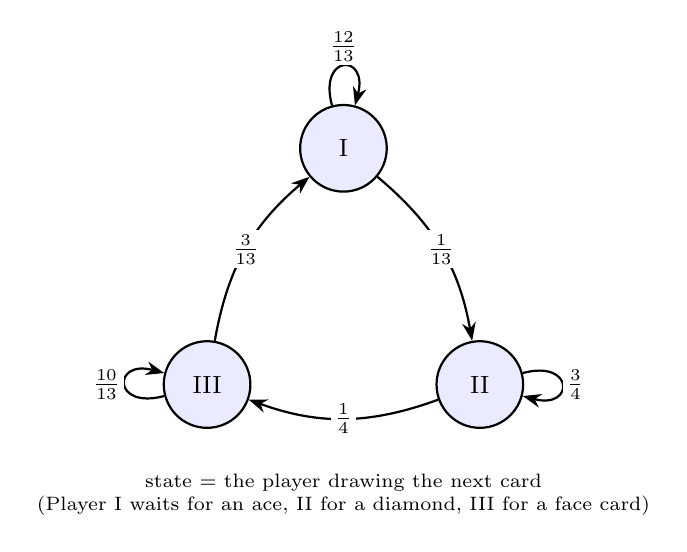
\begin{tikzpicture}[>=Stealth,font=\small,
 s/.style={draw,thick,circle,minimum size=1.1cm,inner sep=0pt,fill=blue!8},
 e/.style={->,thick},
 lab/.style={font=\small,fill=white,inner sep=1.5pt},
 every loop/.style={->,thick,looseness=6}]
\node[s] (1) at (90:2) {I};
\node[s] (2) at (-30:2) {II};
\node[s] (3) at (210:2) {III};
\draw[e] (1) to[bend left=20] node[lab]{$\tfrac{1}{13}$} (2);
\draw[e] (2) to[bend left=20] node[lab]{$\tfrac14$} (3);
\draw[e] (3) to[bend left=20] node[lab]{$\tfrac{3}{13}$} (1);
\path (1) edge[loop above] node[lab]{$\tfrac{12}{13}$} (1);
\path (2) edge[loop right] node[lab]{$\tfrac34$} (2);
\path (3) edge[loop left] node[lab]{$\tfrac{10}{13}$} (3);
\node[font=\scriptsize,align=center] at (0,-2.4) {state = the player drawing the next card\\(Player I waits for an ace, II for a diamond, III for a face card)};
\end{tikzpicture}
\end{document}
